\documentclass{standalone}
\usepackage{tikz}
\usetikzlibrary{bayesnet}

\begin{document}

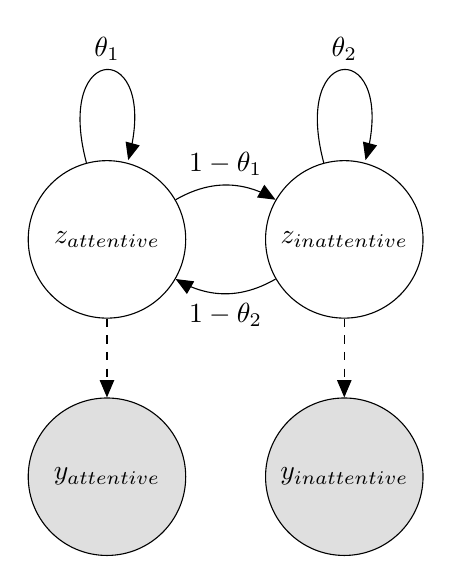
\begin{tikzpicture}[latent/.append style={minimum size=2cm}, obs/.append style={minimum size=2cm}]
  \node[latent] (z0) {$z_{attentive}$};
  \node[latent, right=of z0] (z1) {$z_{inattentive}$};
  \node[obs, below=of z0] (y0) {$y_{attentive}$};
  \node[obs, below=of z1] (y1) {$y_{inattentive}$};

  \edge[dashed] {z0} {y0};
  \edge[dashed] {z1} {y1};
  
  \path (z0) edge[->, >={triangle 45}, loop above] node {$\theta_1$} (z0);
  \path (z1) edge[->, >={triangle 45}, loop above] node {$\theta_2$} (z1);
  \path (z0) edge[->, >={triangle 45}, bend left] node[above] {$1-\theta_1$} (z1);
  \path (z1) edge[->, >={triangle 45}, bend left] node[below] {$1-\theta_2$} (z0);
\end{tikzpicture}

\end{document}
